% user guide(6-10 pages)
\chapter{Ръководство за потребителя}
\hfill

\section{Инсталиране на библиотеката}
        Библиотеката е съвместима с операционната система Linux. 
        Преди да започнете процеса на инсталация ще са Ви нужни следните 
        допълнителни програми:

        \begin{itemize}
                \item git
                \item Python интерпретатор (версия 3.10 или 3.11)
        \end{itemize}

        \subsection{Сдобиване с кода на библиотеката}

                Кодът на програмата може да бъде изтеглен от GitHub хранилището
                на проекта \url{https://github.com/Squidfishrl/tui-framework}.
                Най-удобният и бърз начин е да копирате хранилището директно:

                \begin{lstlisting}[style=shell]
                        $ git clone https://github.com/Squidfishrl/tui-framework
                \end{lstlisting}

                Като алтернатива може да изтеглите кода под формата на zip архив
                \figref{fig:download-zip}:
        
                \begin{figure}[h]
                        \centering
                        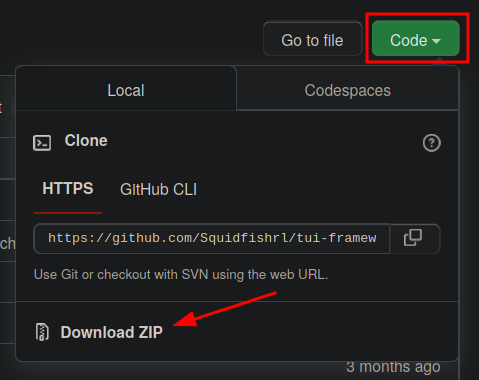
\includegraphics[width=\textwidth]{images/download-zip.png}
                        \caption{Теглене на кода под формата на zip архив}
                        \label{fig:download-zip}
                \end{figure}

        \subsection{Инсталиране на библиотеката}

        След като сте се сдобили с кода може да преминете към инсталацията на 
        библиотеката. Стъпките за това са следните:

        \begin{enumerate}

                \item (по желание) Създайте виртуална среда, за да изолирате
                        библиотеката от общосистемните пакети 
                        \begin{lstlisting}[style=shell]
                                $ mkdir ./venv
                                $ python3 -m venv ./venv
                                $ source ./venv/bin/activate
                        \end{lstlisting}

                \item Инсталирайте пакета и неговите зависимости
                        \begin{lstlisting}[style=shell]
                                $ pip install -e ./tui-framework
                                $ pip install -r requirements.txt
                        \end{lstlisting}

        \end{enumerate}

\section{Ръководство за обучение}

        Най-добрият начин да се научиш да програмираш е, като седнеш да 
        програмираш. В този раздел от ръководството ще имплементираме проста
        програма.

        \subsection{Hello World!}

                Възможно най-простата програма, която можем да напишем е 
                следната: създаваме приложението, използвайки класа 
                \textbf{APP} и го стартираме с \textbf{run} метода.

                \begin{lstlisting}[style=py]
from tui.app import App

app = App()
app.run()
                \end{lstlisting}

                Когато го пуснем, виждаме празен екран с изключение на черен 
                правоъгълник, който следва курсура на мишката ни.
                \figref{fig:app-barebone}:
        
                \vspace{5mm}
                \begin{figure}[h]
                        \centering
                        
\includegraphics[width=150mm]{images/tutorial/basic.png}
                        \caption{}
                        \label{fig:app-barebone}
                \end{figure}
                \vspace{5mm}

                Следващата ни стъпка е да принтираме текста "Hello, World!" на
                екрана. Това се случва посредством класа \textbf{Widget}, а 
                именно \textbf{Label} (надпис).

                \begin{lstlisting}[style=py]
from tui.app import App
from tui.components.label import Label

app = App()
app.root.append_child(
        Label("Hello, World!", style="rows=1, columns=13")
)
app.run()
                \end{lstlisting}

                Както виждаме, за да определим размера на компонента 
                \textbf{Label}, трябва да укажем неговия размер. Това важи за
                всички компоненти в текущата версия на проекта (1.0.0).

                \vspace{5mm}
                \begin{figure}[h]
                        \centering
                        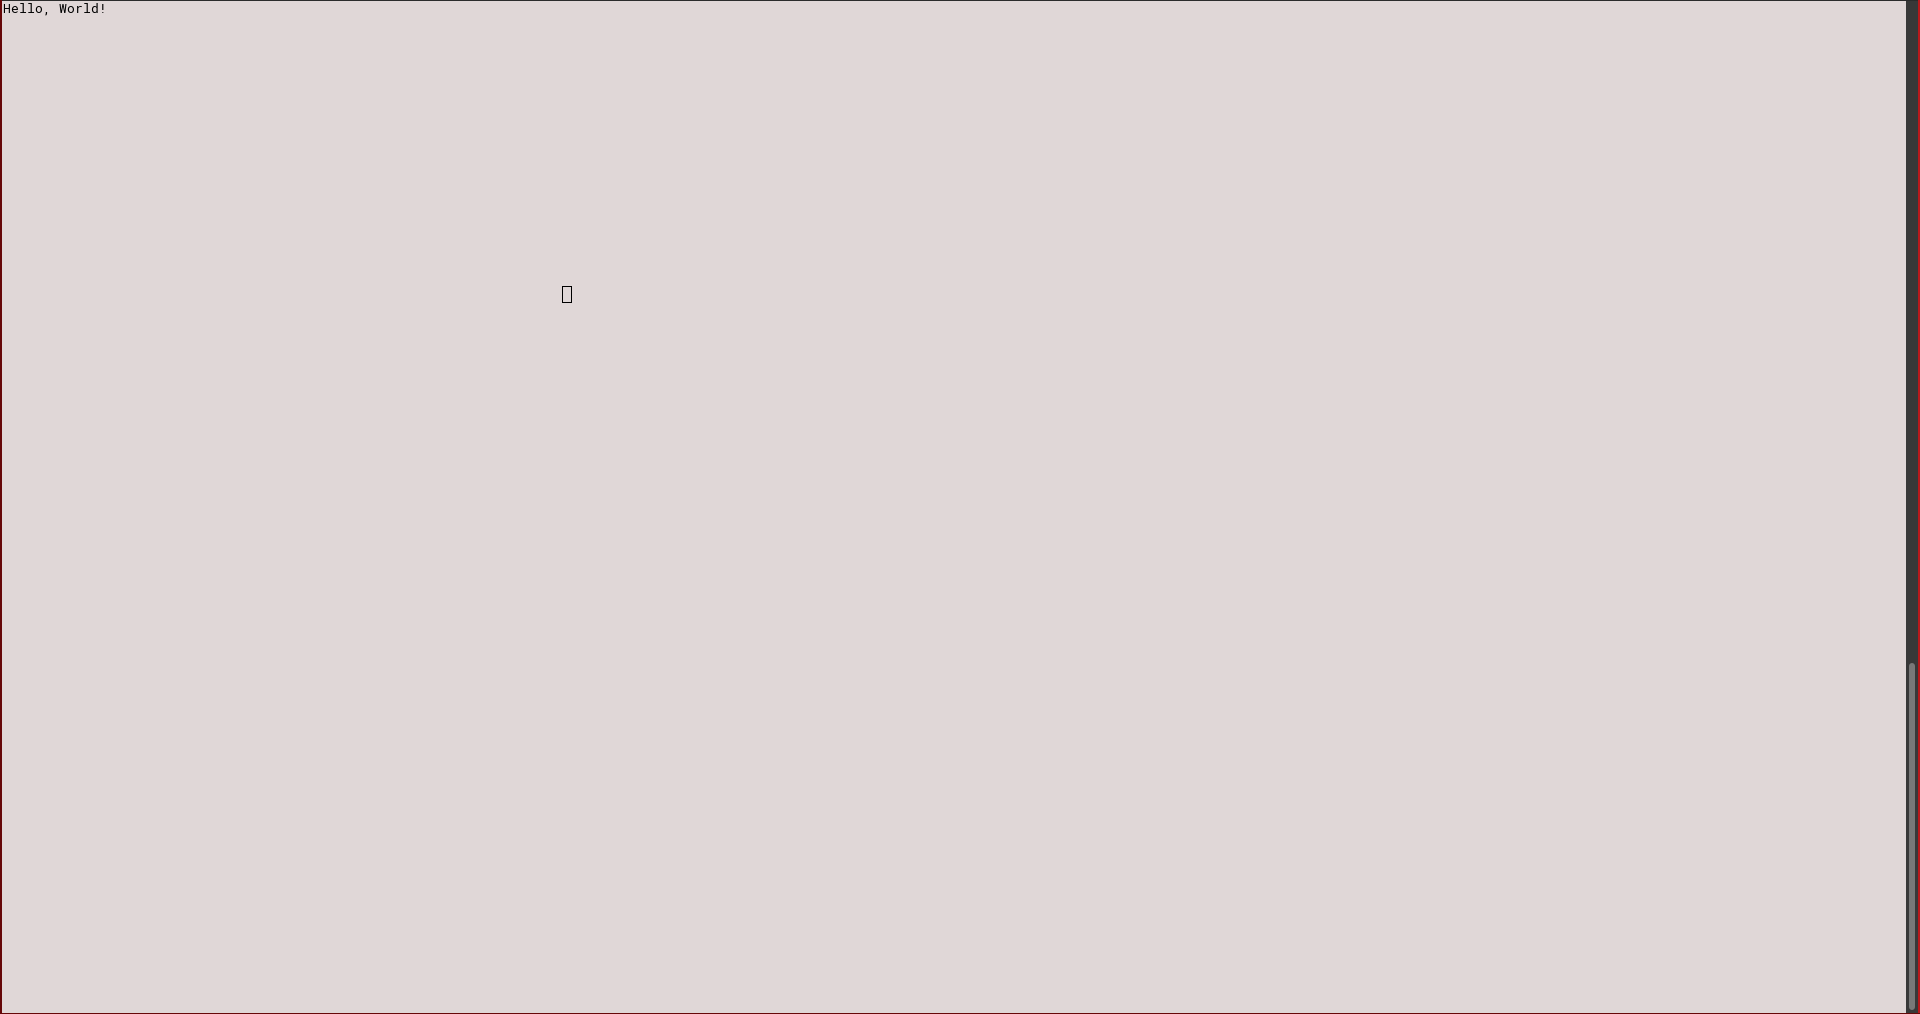
\includegraphics[width=150mm]{images/tutorial/basic-hello-world.png}
                        \caption{}
                        \label{fig:app-bare-hello-world}
                \end{figure}
                \vspace{5mm}

                За да преместим текста \figref{fig:app-bare-hello-world}, в 
                средата на екрата, трябва да разгледаме подпакета 
                \textbf{styles}. Най-лесният начин е да променим размера на 
                надписа и центрираме текста в средата. Друга възможност е да
                използваме \textbf{padding}:

                \begin{lstlisting}[style=py]
from tui.app import App
from tui.components.division import Division
from tui.components.label import Label

app = App()

app.root.set_style("padding", 25)
app.root.append_child(
        Label("Hello, World!", style="rows=1, columns=13")
)

app.run()
                \end{lstlisting}

                \vspace{5mm}
                \begin{figure}[h]
                        \centering
                        
\includegraphics[width=150mm]{images/tutorial/hello-world-padding.png}
                        \caption{}
                        \label{fig:app-hello-world-padding}
                \end{figure}
                \vspace{5mm}

                Може да използваме метода \textbf{add\_border}, за да добавим
                рамка към компонентите:

                \begin{lstlisting}[style=py]
app = App()
root = app.root

root.set_style("margin", 2)

root.append_child(
        Label("Hello, World!", identifier="lbl", style=f"\
                rows={root.area.rows - 2},\
                columns={root.area.columns - 2},\
                text_align=center,\
                vertical_align=center,\
                margin_top={25},\
                margin_bottom={25},\
                margin_left={43},\
                margin_right={43}")
)

root.children.get_by_id("lbl").add_border(DefaultBorder)
root.add_border(DefaultBorder)
app.run()
                \end{lstlisting}

                \vspace{5mm}
                \begin{figure}[h]
                        \centering
                        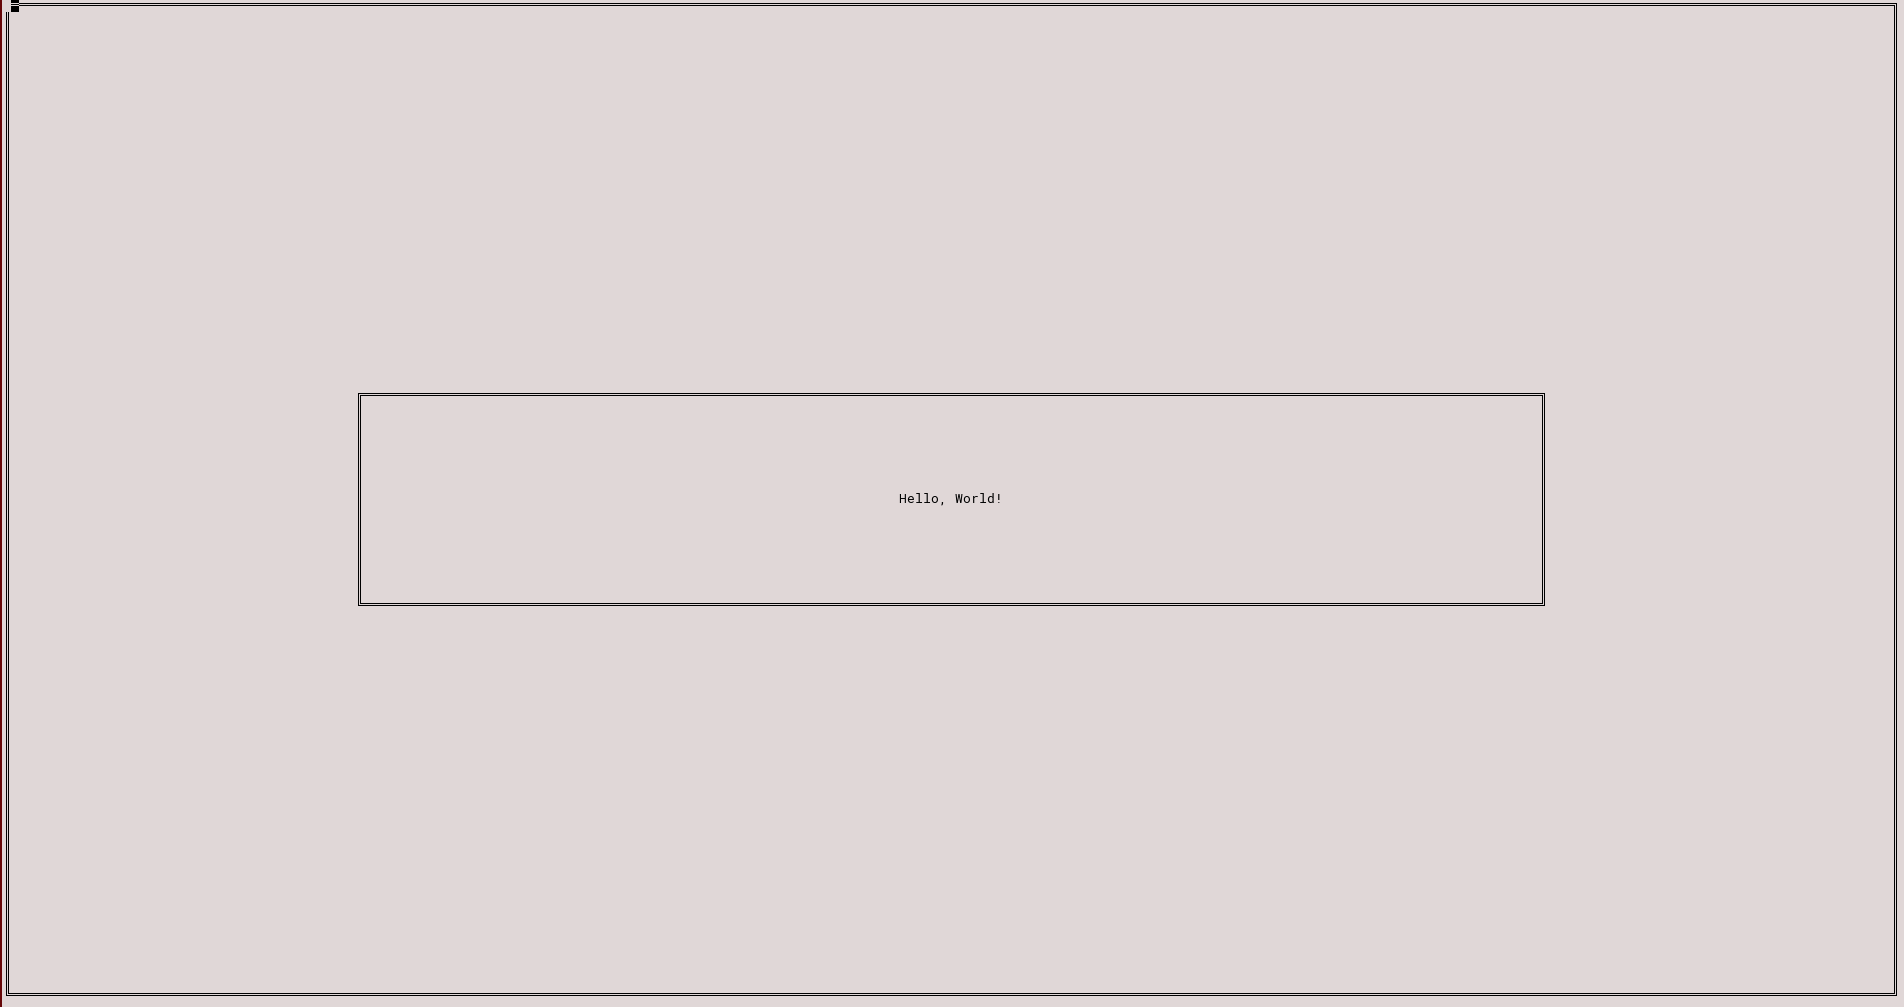
\includegraphics[width=150mm]{images/tutorial/hello-world-center.png}
                        \caption{}
                        \label{fig:hello-world-center}
                \end{figure}
                \vspace{5mm}

                Вече надписът е центриран и заедно с \textbf{root} компонентът 
                има рамка.
                \newline


        Библиотеката има добре описана документация и може да научите много ако 
        разгледате някои от файловете като \textbf{components/widget.py}, 
        \textbf{components/container.py} и \textbf{app.py}. Същевремнно, може
        да разгледате и директорията \textbf{demo}, в която са събрани други
        примери.

